\subsection{Die Übergangsfunktion}

Die Übergangsfunktion, auch Sprungantwort, ist die Antwort im Zeitbereich auf einen Sprung am Eingang von 0 nach 1. \newline
In Abbildung \ref{fig:aufbau} ist der Aufbau zu sehen. Das Oszilloskop in Abbildung \ref{fig:oszilloskop} zeigt die Sprungantwort im Simulationsintervall 0 - 100 an. \newline
In Abbildung \ref{fig:matlab_sprungantwort} ist die Übergangsfunktion in Matlab vom Intervall 0 bis 3500, während Abbildung \ref{fig:matlab100_sprungantwort} die Sprungantwort im Intervall 0 bis 100 zeigt. 

\begin{figure}[H]
	\centering
	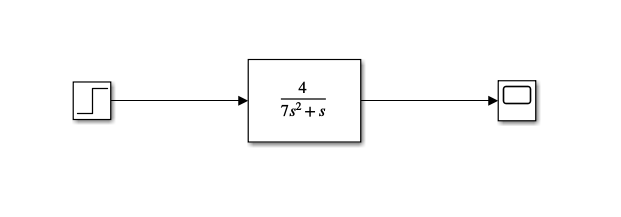
\includegraphics[width=0.8\textwidth]{{diagrams/aufbau.png}}
	\caption[Aufbau]{Aufbau in Simulink}
	\label{fig:aufbau}
\end{figure}

\begin{figure}[H]
	\centering
	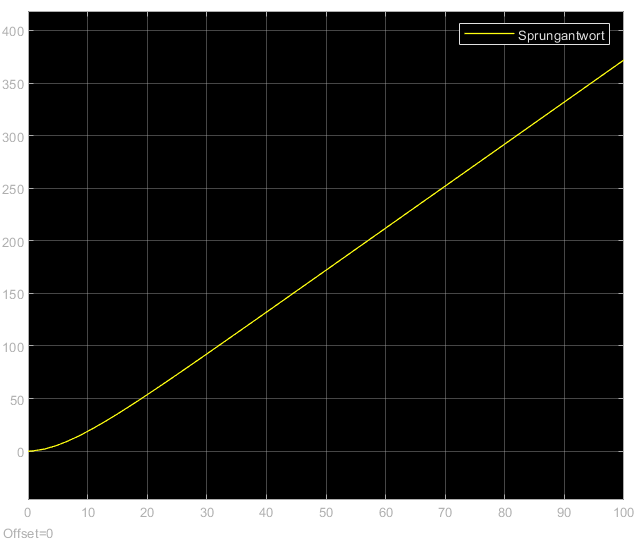
\includegraphics[width=0.8\textwidth]{{diagrams/sprungantwort_simulink_100.png}}
	\caption[Oszilloskop]{Oszilloskop - Sprungantwort im Intervall 0 bis 100}
	\label{fig:oszilloskop}
\end{figure}

\begin{figure}[H]
	\centering
	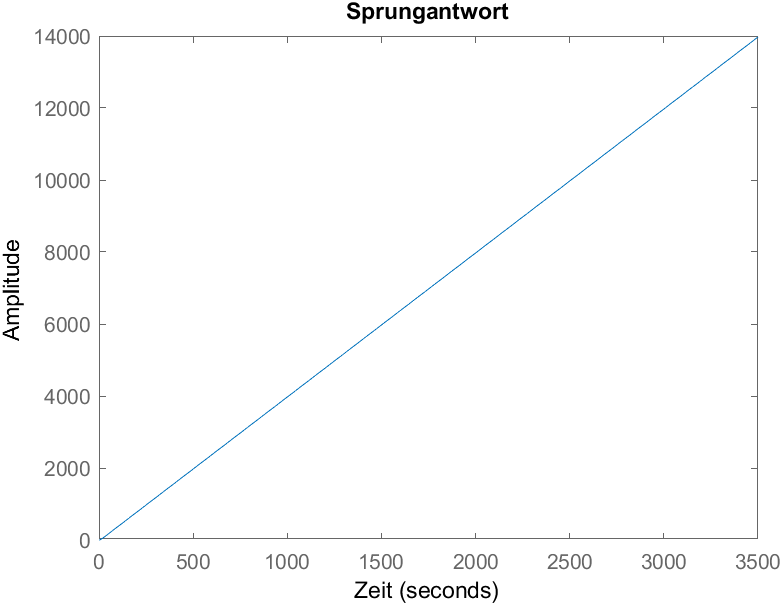
\includegraphics[width=0.8\textwidth]{{diagrams/sprungantwort_matlab.png}}
	\caption[Oszilloskop]{Matlab - Sprungantwort}
	\label{fig:matlab_sprungantwort}
\end{figure}

\begin{figure}[H]
	\centering
	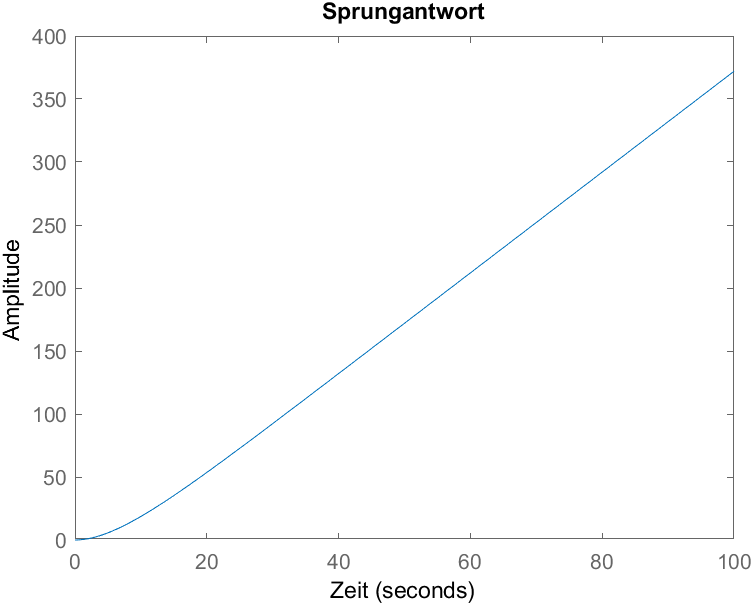
\includegraphics[width=0.8\textwidth]{{diagrams/sprungantwort_matlab_limit100.png}}
	\caption[Oszilloskop]{Matlab - Sprungantwort im Intervall 0 bis 100}
	\label{fig:matlab100_sprungantwort}
\end{figure}